% Practice Test 08 — Minnesota Edition
% Questions: 30 (21 MC + 9 SA)
% Generated by scripts/generate_practice_tests.py

\begin{practiceQuestion}{1-3-q13}{mc}
\begin{questionText}
The table shows a proportional relationship. Find the missing value.

\begin{center}
\begin{tabular}{|c|c|}
\hline $x$ & $y$ \\ \hline $4$ & $14$ \\ $6$ & $?$ \\ $10$ & $35$ \\ \hline
\end{tabular}
\end{center}
\end{questionText}
\choiceA{$18$}
\choiceB{$20$}
\choiceC{$21$}
\choiceD{$24$}
\correctAnswer{C}
\explanation{$k = \frac{14}{4} = 3.5$. Missing value: $y = 3.5 \times 6 = 21$. Check: $\frac{35}{10} = 3.5$ \checkmark.}
\end{practiceQuestion}

\begin{practiceQuestion}{1-5-q21}{sa}
\begin{questionText}
A proportional line has slope $\frac{5}{3}$. Find $y$ when $x = 9$ and $x$ when $y = 25$.
\end{questionText}
\correctAnswer{$y = 15$ when $x = 9$; $x = 15$ when $y = 25$}
\explanation{$y = \frac{5}{3} \times 9 = 15$. For $y = 25$: $25 = \frac{5}{3}x$, so $x = 25 \times \frac{3}{5} = 15$.}
\end{practiceQuestion}

\begin{practiceQuestion}{1-6-q26}{gmc}
\begin{questionText}
The table shows the distance a bus travels over several hours. Using proportional reasoning, how far will the bus travel in $9$ hours?

\begin{center}
\begin{tabular}{|c|c|}
\hline
\textbf{Hours} & \textbf{Miles} \\ \hline
$2$ & $90$ \\ \hline
$5$ & $225$ \\ \hline
$7$ & $315$ \\ \hline
$9$ & $?$ \\ \hline
\end{tabular}
\end{center}
\end{questionText}
\choiceA{$360$ miles}
\choiceB{$385$ miles}
\choiceC{$405$ miles}
\choiceD{$450$ miles}
\correctAnswer{C}
\explanation{Rate: $90 \div 2 = 45$ mph. In $9$ hours: $45 \times 9 = 405$ miles.}
\end{practiceQuestion}

\begin{practiceQuestion}{2-1-q10}{mc}
\begin{questionText}
What is $8\%$ of $250$?
\end{questionText}
\choiceA{$2$}
\choiceB{$16$}
\choiceC{$20$}
\choiceD{$32$}
\correctAnswer{C}
\explanation{$8\% = 0.08$. Multiply: $0.08 \times 250 = 20$.}
\end{practiceQuestion}

\begin{practiceQuestion}{2-5-q17}{mc}
\begin{questionText}
A freelance artist charges a $\$50$ base fee plus $7\%$ of the project value. For a $\$600$ project, what is the total charge?


\numberLine[100]{0}{700}
\end{questionText}
\choiceA{$\$42$}
\choiceB{$\$92$}
\choiceC{$\$107$}
\choiceD{$\$650$}
\correctAnswer{B}
\explanation{Percent fee: $600 \times 0.07 = \$42$. Total: $50 + 42 = \$92$.}
\end{practiceQuestion}

\begin{practiceQuestion}{2-7-q27}{gmc}
\begin{questionText}
The bar graph shows the estimated and actual heights of three trees. Which tree has the greatest percent error?

\begin{center}
\begin{tikzpicture}[scale=0.5]
  \draw[thick,->] (0,0) -- (0,7) node[above]{\small Height (ft)};
  \draw[thick,->] (0,0) -- (10.5,0);
  % Tree A: est 20, actual 25
  \fill[funBlue!60] (0.5,0) rectangle (1.5,4);
  \fill[funGreen!60] (1.5,0) rectangle (2.5,5);
  % Tree B: est 15, actual 12
  \fill[funBlue!60] (3.5,0) rectangle (4.5,3);
  \fill[funGreen!60] (4.5,0) rectangle (5.5,2.4);
  % Tree C: est 30, actual 28
  \fill[funBlue!60] (6.5,0) rectangle (7.5,6);
  \fill[funGreen!60] (7.5,0) rectangle (8.5,5.6);
  % Labels
  \node[below,font=\small] at (1.5,0) {Tree A};
  \node[below,font=\small] at (4.5,0) {Tree B};
  \node[below,font=\small] at (7.5,0) {Tree C};
  \foreach \y/\lab in {1/5,2/10,3/15,4/20,5/25,6/30} {
    \draw (-0.1,\y) -- (0.1,\y) node[left,font=\small,xshift=-2pt] {\lab};
  }
  % Values
  \node[above,font=\scriptsize,funBlue] at (1,4) {$20$};
  \node[above,font=\scriptsize,funGreen!80!black] at (2,5) {$25$};
  \node[above,font=\scriptsize,funBlue] at (4,3) {$15$};
  \node[above,font=\scriptsize,funGreen!80!black] at (5,2.4) {$12$};
  \node[above,font=\scriptsize,funBlue] at (7,6) {$30$};
  \node[above,font=\scriptsize,funGreen!80!black] at (8,5.6) {$28$};
  % Legend
  \fill[funBlue!60] (0.5,6.8) rectangle (1,7.2);
  \node[right,font=\scriptsize] at (1.1,7) {Estimated};
  \fill[funGreen!60] (3.5,6.8) rectangle (4,7.2);
  \node[right,font=\scriptsize] at (4.1,7) {Actual};
\end{tikzpicture}
\end{center}
\end{questionText}
\choiceA{Tree A ($20\%$)}
\choiceB{Tree B ($25\%$)}
\choiceC{Tree C ($7.1\%$)}
\choiceD{Trees A and B are tied}
\correctAnswer{B}
\explanation{A: $|20-25|/25 = 20\%$. B: $|15-12|/12 = 25\%$. C: $|30-28|/28 \approx 7.1\%$. Tree B has the greatest error.}
\end{practiceQuestion}

\begin{practiceQuestion}{2-8-q04}{mc}
\begin{questionText}
You buy a $\$500$ laptop using a credit card at $12\%$ annual interest. If you pay it all back after $1$ year, what is the total cost?
\end{questionText}
\choiceA{$\$512$}
\choiceB{$\$560$}
\choiceC{$\$600$}
\choiceD{$\$550$}
\correctAnswer{B}
\explanation{Interest $= 500 \times 0.12 \times 1 = \$60$. Total $= 500 + 60 = \$560$.}
\end{practiceQuestion}

\begin{practiceQuestion}{3-1-q12}{mc}
\begin{questionText}
The temperature at noon was $5°$C. By midnight it was $-5°$C. What is the relationship between these temperatures?
\end{questionText}
\choiceA{They are equal}
\choiceB{They are opposites}
\choiceC{Midnight was warmer}
\choiceD{Their absolute values are different}
\correctAnswer{B}
\explanation{$5$ and $-5$ are the same distance from $0$ but on opposite sides of the number line. They are opposites.}
\end{practiceQuestion}

\begin{practiceQuestion}{4-1-q25}{sa}
\begin{questionText}
A student earns $\$8.50$ per hour at a part-time job. Write an expression for the weekly earnings if the student works $h$ hours, and find the earnings for a $20$-hour week.
\end{questionText}
\correctAnswer{$8.50h$; $\$170$}
\explanation{Weekly earnings: $8.50h$. For $h = 20$: $8.50(20) = \$170$.}
\end{practiceQuestion}

\begin{practiceQuestion}{4-2-q03}{mc}
\begin{questionText}
Simplify $9a - 4a + 6$.
\end{questionText}
\choiceA{$11a$}
\choiceB{$5a + 6$}
\choiceC{$5a - 6$}
\choiceD{$13a - 4$}
\correctAnswer{B}
\explanation{Combine $9a - 4a = 5a$. The constant $6$ stays. Result: $5a + 6$.}
\end{practiceQuestion}

\begin{practiceQuestion}{5-2-q30}{gsa}
\begin{questionText}
The flowchart shows the steps used to get from $x$ to $22$. Work backward to find $x$.

\begin{center}
\begin{tikzpicture}[node distance=2cm, auto, scale=0.8]
  \node[draw,rounded corners,fill=funBlue!15,minimum width=1.5cm] (start) {$x$};
  \node[draw,fill=funOrange!15,minimum width=1.5cm,right of=start] (step1) {$\times 5$};
  \node[draw,fill=funOrange!15,minimum width=1.5cm,right of=step1] (step2) {$- 3$};
  \node[draw,rounded corners,fill=funGreen!15,minimum width=1.5cm,right of=step2] (end) {$22$};
  \draw[->,thick] (start) -- (step1);
  \draw[->,thick] (step1) -- (step2);
  \draw[->,thick] (step2) -- (end);
\end{tikzpicture}
\end{center}
\end{questionText}
\correctAnswer{$x = 5$}
\explanation{The equation is $5x - 3 = 22$. Add $3$: $5x = 25$. Divide by $5$: $x = 5$. Check: $5 \times 5 = 25$, $25 - 3 = 22$ \checkmark.}
\end{practiceQuestion}

\begin{practiceQuestion}{5-3-q19}{sa}
\begin{questionText}
Solve $4(x + 9) = 52$.
\end{questionText}
\correctAnswer{$x = 4$}
\explanation{Divide by $4$: $x + 9 = 13$. Subtract $9$: $x = 4$. Check: $4(4 + 9) = 4(13) = 52$ \checkmark.}
\end{practiceQuestion}

\begin{practiceQuestion}{5-4-q21}{sa}
\begin{questionText}
Solve $\dfrac{x}{2} + \dfrac{x}{4} = 9$.
\end{questionText}
\correctAnswer{$x = 12$}
\explanation{Multiply every term by $4$: $2x + x = 36$. Combine: $3x = 36$. Divide by $3$: $x = 12$. Check: $\frac{12}{2} + \frac{12}{4} = 6 + 3 = 9$ \checkmark.}
\end{practiceQuestion}

\begin{practiceQuestion}{5-5-q07}{mc}
\begin{questionText}
You have $\$60$ and spend $\$8$ per day. You want to have at least $\$12$ left. Which inequality finds the number of days $d$ you can spend?
\end{questionText}
\choiceA{$60 - 8d \leq 12$}
\choiceB{$60 + 8d \geq 12$}
\choiceC{$60 - 8d \geq 12$}
\choiceD{$8d - 60 \geq 12$}
\correctAnswer{C}
\explanation{Start with $\$60$, subtract $\$8$ per day, need at least $\$12$: $60 - 8d \geq 12$.}
\end{practiceQuestion}

\begin{practiceQuestion}{5-6-q02}{mc}
\begin{questionText}
Which graph represents $x \leq -2$?
\end{questionText}
\choiceA{Open circle at $-2$, shade left}
\choiceB{Closed circle at $-2$, shade right}
\choiceC{Closed circle at $-2$, shade left}
\choiceD{Open circle at $-2$, shade right}
\correctAnswer{C}
\explanation{$x \leq -2$: closed circle (includes $-2$) and shade left (values less than or equal to $-2$).}
\end{practiceQuestion}

\begin{practiceQuestion}{6-3-q24}{sa}
\begin{questionText}
You are given angles $45°$ and $45°$ and side $6$ cm between them. How many triangles can you draw?
\end{questionText}
\correctAnswer{Exactly one}
\explanation{ASA (two angles and the included side) fully determine a unique triangle. The third angle would be $180° - 45° - 45° = 90°$.}
\end{practiceQuestion}

\begin{practiceQuestion}{6-4-q28}{gmc}
\begin{questionText}
The diagram shows two triangles. Both have angles $30°$, $60°$, and $90°$, but different side lengths. What does this demonstrate?

\begin{center}
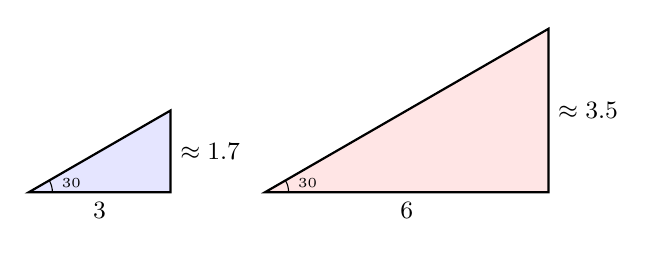
\begin{tikzpicture}[scale=0.6]
  % Small triangle
  \draw[thick,fill=blue!10] (0,0) -- (3,0) -- (3,1.73) -- cycle;
  \node[below] at (1.5,0) {\small $3$};
  \node[right] at (3,0.86) {\small $\approx 1.7$};
  \draw (0.5,0) arc[start angle=0,end angle=30,radius=0.5];
  \node at (0.9,0.2) {\tiny $30°$};
  % Large triangle
  \draw[thick,fill=red!10] (5,0) -- (11,0) -- (11,3.46) -- cycle;
  \node[below] at (8,0) {\small $6$};
  \node[right] at (11,1.73) {\small $\approx 3.5$};
  \draw (5.5,0) arc[start angle=0,end angle=30,radius=0.5];
  \node at (5.9,0.2) {\tiny $30°$};
\end{tikzpicture}
\end{center}
\end{questionText}
\choiceA{SSS produces multiple triangles}
\choiceB{AAA produces a unique triangle}
\choiceC{AAA produces multiple triangles of different sizes}
\choiceD{These two triangles are congruent}
\correctAnswer{C}
\explanation{Both triangles have the same angles but different side lengths. AAA determines shape but not size, so many triangles are possible.}
\end{practiceQuestion}

\begin{practiceQuestion}{6-5-q15}{mc}
\begin{questionText}
A pyramid with a square base is sliced with a horizontal cut near the top. What shape is the cross-section?
\end{questionText}
\choiceA{A very small square}
\choiceB{A triangle}
\choiceC{A point}
\choiceD{A circle}
\correctAnswer{A}
\explanation{A horizontal cut of a square pyramid parallel to the base gives a square. Near the top, the square is very small. At the very apex it would be a point, but a cut ``near the top'' gives a small square.}
\end{practiceQuestion}

\begin{practiceQuestion}{6-6-q04}{mc}
\begin{questionText}
Two supplementary angles are $(2x + 10)°$ and $(3x)°$. What is the value of $x$?
\end{questionText}
\choiceA{$30$}
\choiceB{$34$}
\choiceC{$36$}
\choiceD{$40$}
\correctAnswer{B}
\explanation{$2x + 10 + 3x = 180$. Combine: $5x + 10 = 180$. Subtract $10$: $5x = 170$. Divide: $x = 34$.}
\end{practiceQuestion}

\begin{practiceQuestion}{7-3-q17}{mc}
\begin{questionText}
What is the area of a circle with a radius of $1.5$ meters? Use $\pi \approx 3.14$.
\end{questionText}
\choiceA{$4.71$ m$^2$}
\choiceB{$7.065$ m$^2$}
\choiceC{$9.42$ m$^2$}
\choiceD{$14.13$ m$^2$}
\correctAnswer{B}
\explanation{$A = \pi r^2 = 3.14 \times (1.5)^2 = 3.14 \times 2.25 = 7.065$ m$^2$.}
\end{practiceQuestion}

\begin{practiceQuestion}{7-4-q26}{gmc}
\begin{questionText}
What is the area of the shaded composite figure on the grid? Each square is $1$ cm by $1$ cm.

\begin{center}
\begin{tikzpicture}[scale=0.5]
  \draw[step=1,gray!30,thin] (0,0) grid (10,7);
  \fill[funBlue!20] (1,1) -- (9,1) -- (9,4) -- (6,4) -- (6,6) -- (4,6) -- (4,4) -- (1,4) -- cycle;
  \draw[thick,funBlue] (1,1) -- (9,1) -- (9,4) -- (6,4) -- (6,6) -- (4,6) -- (4,4) -- (1,4) -- cycle;
  \node[below] at (1,1) {\small $(1{,}1)$};
  \node[below] at (9,1) {\small $(9{,}1)$};
  \node[right] at (9,4) {\small $(9{,}4)$};
  \node[right] at (6,4) {\small $(6{,}4)$};
  \node[above] at (6,6) {\small $(6{,}6)$};
  \node[above] at (4,6) {\small $(4{,}6)$};
  \node[left] at (4,4) {\small $(4{,}4)$};
  \node[left] at (1,4) {\small $(1{,}4)$};
\end{tikzpicture}
\end{center}
\end{questionText}
\choiceA{$24$ cm$^2$}
\choiceB{$28$ cm$^2$}
\choiceC{$32$ cm$^2$}
\choiceD{$36$ cm$^2$}
\correctAnswer{B}
\explanation{Bottom rectangle: $8 \times 3 = 24$ cm$^2$. Top rectangle: $2 \times 2 = 4$ cm$^2$. Total: $24 + 4 = 28$ cm$^2$.}
\end{practiceQuestion}

\begin{practiceQuestion}{7-5-q20}{sa}
\begin{questionText}
A cube has a side length of $7$ m. What is its surface area?
\end{questionText}
\correctAnswer{$294$ m$^2$}
\explanation{$SA = 6s^2 = 6 \times 49 = 294$ m$^2$.}
\end{practiceQuestion}

\begin{practiceQuestion}{7-6-q16}{mc}
\begin{questionText}
A rectangular prism has a volume of $240$ cm$^3$. Its base is $8$ cm by $6$ cm. What is the height?
\end{questionText}
\choiceA{$4$ cm}
\choiceB{$5$ cm}
\choiceC{$6$ cm}
\choiceD{$10$ cm}
\correctAnswer{B}
\explanation{$B = 8 \times 6 = 48$ cm$^2$. $h = V \div B = 240 \div 48 = 5$ cm.}
\end{practiceQuestion}

\begin{practiceQuestion}{8-1-q30}{gsa}
\begin{questionText}
The table shows the results of a random sample of $80$ people about their preferred pet.

\begin{center}
\begin{tabular}{|l|c|}
\hline
\textbf{Pet} & \textbf{Number} \\
\hline
Dog & $32$ \\
\hline
Cat & $24$ \\
\hline
Fish & $12$ \\
\hline
Bird & $8$ \\
\hline
Other & $4$ \\
\hline
\end{tabular}
\end{center}

What percent of the sample prefers cats? If the population is $5{,}000$, predict how many prefer cats.
\end{questionText}
\correctAnswer{$30\%$; $1{,}500$ people}
\explanation{$\frac{24}{80} = 0.30 = 30\%$. Then $30\%$ of $5{,}000 = 1{,}500$.}
\end{practiceQuestion}

\begin{practiceQuestion}{8-3-q01}{mc}
\begin{questionText}
Class A has a mean test score of $78$ and Class B has a mean test score of $85$. What can you conclude?
\end{questionText}
\choiceA{Every student in Class B scored higher than every student in Class A}
\choiceB{Class B scored higher on average than Class A}
\choiceC{Class A and Class B have the same scores}
\choiceD{Class A has more students than Class B}
\correctAnswer{B}
\explanation{The mean tells us the average performance. Class B scored higher on average, but individual scores may overlap.}
\end{practiceQuestion}

\begin{practiceQuestion}{8-4-q14}{mc}
\begin{questionText}
Data: $42, 45, 47, 50, 53, 55, 58$. Find $Q_1$ and $Q_3$.
\end{questionText}
\choiceA{$Q_1 = 45$, $Q_3 = 55$}
\choiceB{$Q_1 = 42$, $Q_3 = 58$}
\choiceC{$Q_1 = 47$, $Q_3 = 53$}
\choiceD{$Q_1 = 44$, $Q_3 = 56$}
\correctAnswer{A}
\explanation{Median $= 50$. Lower half: $42, 45, 47$, so $Q_1 = 45$. Upper half: $53, 55, 58$, so $Q_3 = 55$.}
\end{practiceQuestion}

\begin{practiceQuestion}{8-6-q03}{mc}
\begin{questionText}
A sector of a circle graph represents $25\%$ of the data. What is its angle?
\end{questionText}
\choiceA{$25°$}
\choiceB{$45°$}
\choiceC{$90°$}
\choiceD{$180°$}
\correctAnswer{C}
\explanation{$25\% \times 360° = 0.25 \times 360° = 90°$.}
\end{practiceQuestion}

\begin{practiceQuestion}{9-4-q21}{sa}
\begin{questionText}
A bag has $6$ red, $4$ blue, and $10$ white marbles. Write the probability model by listing $P(\text{red})$, $P(\text{blue})$, and $P(\text{white})$ as fractions in simplest form.
\end{questionText}
\correctAnswer{$P(\text{red}) = \frac{3}{10}$, $P(\text{blue}) = \frac{1}{5}$, $P(\text{white}) = \frac{1}{2}$}
\explanation{Total: $20$. $P(\text{red}) = \frac{6}{20} = \frac{3}{10}$, $P(\text{blue}) = \frac{4}{20} = \frac{1}{5}$, $P(\text{white}) = \frac{10}{20} = \frac{1}{2}$.}
\end{practiceQuestion}

\begin{practiceQuestion}{9-6-q26}{gmc}
\begin{questionText}
The table shows all possible sums when two dice are rolled. What is the probability of rolling a sum of $8$?

\begin{center}
\begin{tabular}{|c|c|c|c|c|c|c|}
\hline
$+$ & \textbf{1} & \textbf{2} & \textbf{3} & \textbf{4} & \textbf{5} & \textbf{6} \\
\hline
\textbf{1} & $2$ & $3$ & $4$ & $5$ & $6$ & $7$ \\
\hline
\textbf{2} & $3$ & $4$ & $5$ & $6$ & $7$ & \cellcolor{funBlue!20}$8$ \\
\hline
\textbf{3} & $4$ & $5$ & $6$ & $7$ & \cellcolor{funBlue!20}$8$ & $9$ \\
\hline
\textbf{4} & $5$ & $6$ & $7$ & \cellcolor{funBlue!20}$8$ & $9$ & $10$ \\
\hline
\textbf{5} & $6$ & $7$ & \cellcolor{funBlue!20}$8$ & $9$ & $10$ & $11$ \\
\hline
\textbf{6} & $7$ & \cellcolor{funBlue!20}$8$ & $9$ & $10$ & $11$ & $12$ \\
\hline
\end{tabular}
\end{center}
\end{questionText}
\choiceA{$\frac{4}{36}$}
\choiceB{$\frac{5}{36}$}
\choiceC{$\frac{6}{36}$}
\choiceD{$\frac{8}{36}$}
\correctAnswer{B}
\explanation{Outcomes with sum $8$: $(2,6), (3,5), (4,4), (5,3), (6,2)$ — that is $5$. $P = \frac{5}{36}$.}
\end{practiceQuestion}

\begin{practiceQuestion}{9-7-q18}{mc}
\begin{questionText}
In a simulation of $100$ free throws, a basketball player makes $78$. If the player's actual success rate is $75\%$, is the simulation result reasonable?
\end{questionText}
\choiceA{No, any difference means the simulation is wrong}
\choiceB{Yes, $78\%$ is close to $75\%$, which is expected variation}
\choiceC{No, because $78$ is not equal to $75$}
\choiceD{Yes, but only if exactly $75$ are made}
\correctAnswer{B}
\explanation{$\frac{78}{100} = 0.78$ vs. theoretical $0.75$. A small difference in $100$ trials is normal and expected.}
\end{practiceQuestion}
